\scanpage{17}
$x$ en question, ou les $i$ en question) forment un \uline{torseur} sous le groupe $\handwritten{Z^+}=$\deleted{$\handwritten{\unsure{U\cap}}\operatorname{Cent}(u)$}\inserted{$\handwritten{Z\cap U}$},
% The cancelled interlinear note has a curved enclosure continuing into a leader.
% Its left endpoint is near the punctuation after unipotent; no exact glyph attachment is imposed.
\figure{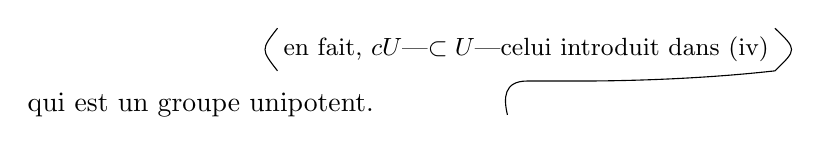
\begin{tikzpicture}[x=1cm,y=1cm]
  \node[anchor=west,inner sep=0pt] (body) at (0,0) {qui est un groupe unipotent\handwritten{.}};
  \node[anchor=west,inner sep=0pt,font=\small] (note) at (3.25,.70) {\handwritten{\deleted{en fait, \unsure{$cU$|$\subset U$|celui} introduit dans (iv)}}};
  \draw[line width=.4pt] ([xshift=-2pt,yshift=3pt]note.north west) .. controls ([xshift=-8pt]note.west) .. ([xshift=-2pt,yshift=-3pt]note.south west);
  \draw[line width=.4pt] ([xshift=2pt,yshift=3pt]note.north east) .. controls ([xshift=10pt]note.east) .. ([xshift=2pt,yshift=-3pt]note.south east)
    .. controls (8.7,.34) and (7.8,.30) .. (7.0,.30)
    -- (6.35,.30) .. controls (6.05,.30) and (6.05,.08) .. (6.10,-.13);
\end{tikzpicture}}
\margin{\handwritten{%
% margin note written slanted; the source line positions and split semi-direct are retained.
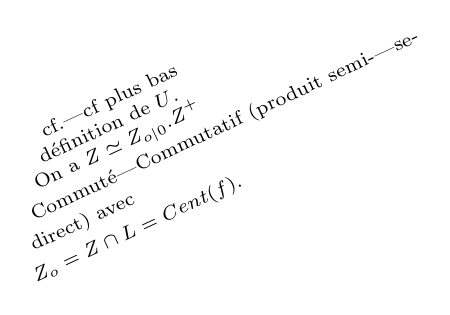
\begin{tikzpicture}[x=.65cm,y=.65cm,every node/.style={anchor=west,inner sep=0pt,font=\scriptsize,rotate=25}]
  \node at (.08,2.85) {\unsure{cf.|cf} plus bas};
  \node at (.02,2.37) {définition de $U$.};
  \node at (-.06,1.84) {On a $Z\simeq Z_{\unsure{o|0}}.Z^+$};
  \node at (-.12,1.22) {\deleted{\unsure{Commuté|Commutatif}} (produit \unsure{semi-|se-}};
  \node at (-.13,.63) {direct) avec};
  \node at (-.08,.02) {$Z_o=Z\cap L=\operatorname{Cent}(f)$.};
\end{tikzpicture}}}
Enfin, supposant toujours $e\handwritten{\ne}0$, l'ensemble des $x$ en question est un torseur sous \deleted{$\handwritten{\unsure{\mathfrak{g}|\mathscr{G}}}^{e}=$ (centralisateur de $e$ \deleted{\unsure{dans}} dans $\handwritten{\mathfrak{g}}$)$=\operatorname{Ker}\operatorname{ad}(e)=\operatorname{Lie}\operatorname{Cent}(u)$}\inserted{$\handwritten{\operatorname{Lie}(Z^+)=\mathfrak{g}^{e}\cap\operatorname{Fil}^{1}(\mathfrak{g})}$} (\inserted{\handwritten{torseur}}pour l'addition, i.e. est de la forme $a+\handwritten{\mathfrak{g}}^e$, pour un $a\handwritten{\in\mathfrak{g}}$ convenable)\handwritten{.} \deleted{(et on a $\handwritten{\mathfrak{g}^{e}\subset\sum_{k\geq1}\mathfrak{g}}(k)=\operatorname{Fil}^{1}\handwritten{\unsure{(\mathfrak{g})|\mathfrak{g}}}$)}

(iii) Soit $x\inserted{\handwritten{\ne0}}$ un élément de Dynkin de $\handwritten{\mathfrak{g}}$, donc associé à un homomorphisme de Dynkin $i:\underline{G}_m\handwritten{\longrightarrow}G$. Alors les éléments\inserted{\handwritten{$e$}} de $\handwritten{\mathfrak{g}}$ tels que $(x,e)$ satisfasse\deleted{nt} aux conditions de (i) forment un ouvert dense\inserted{\handwritten{\deleted{$\unsure{\mathfrak{g}(2)^*}$}}} de $\handwritten{\mathfrak{g}}(2)$ (savoir l'ouvert\inserted{\handwritten{$\mathfrak{g}(2)^*$}} des points $e$ tels que $\operatorname{ad}(e):\handwritten{\mathfrak{g}}(0)\handwritten{\to\mathfrak{g}}(2)$ soit surjectif), \deleted{qui}\inserted{Celui\unsure{\begin{tikzpicture}[baseline=(h.base)]\node[inner sep=0pt] (h) {-};\node[inner sep=0pt] at (h.center) {(};\end{tikzpicture}}ci} est un \deleted{\uline{torseur}}\inserted{\handwritten{espace homogène}} sous\inserted{\handwritten{$L=$}}$\operatorname{Cent}(x)=\operatorname{Cent}(i)$, qui est un groupe réductif.
% The sign between Celui and ci has a horizontal hyphen and a full curved left-parenthesis-like stroke at the same position; their order is unresolved.

(iv) Bour tout \deleted{couple $(x,e)$ satisfaisant les conditions de (i)\unsure{,}}\inserted{élément de Dynkin $x$ de $\handwritten{\mathfrak{g}}$, $x=\operatorname{Lie}(i)(1)$,} considérons les sous-groupes $P,U,\inserted{L}$ de $G$ définis par les conditions
\[
\operatorname{Lie}P=\handwritten{\sum_{k\geq0}\mathfrak{g}}(k)\quad,\quad
\operatorname{Lie}U=\handwritten{\sum}_{k\handwritten{\geq}\deleted{0}\handwritten{1}}\handwritten{\mathfrak{g}}(k),\quad
\operatorname{Lie}L=\handwritten{\mathfrak{g}}(0).
\]
Alors $P$ est un sous-groupe parabolique de $G$, $U$ est son radical unipotent, et $L=\operatorname{Cent}(x)=\operatorname{Cent}(i)$ \deleted{\unsure{en|un}} est un sous-groupe de Lévi de $G$. Si $\unsure{u|a}\inserted{=\exp(e)}$ est un élément unipotent de $G$ tel que $(i,u)$ soit un couple de Dynkin (i.e. induit par un $f:\unsure{\operatorname{SZ}|\operatorname{Sl}}(2,k)\handwritten{\to}G$), $P$ (donc \unsure{aassi|aussi} $U$) est défini en termes de $u$ (i.e; deux $x$ associés au même $u$ donnent le même $P$, cf. (ii)); il en est de même du sous-groupe $H=i(\underline{G}_m).U$ de $G$ (NB $i(\underline{G}_m)$ normalise $U$, et $H$ est un produit semi-direct), et de $i$ mod $U$ i.e. de $\underline{G}_m\handwritten{\longrightarrow}H/U$ induit par $i$. \deleted{\unsure{A}}De plus, l'application
\[
g\handwritten{\longmapsto}\operatorname{ad}(g).x
\]
est un\deleted{e} isomorphisme de $U$ avec $x+\operatorname{Fil}^{1}\handwritten{\mathfrak{g}}\inserted{\handwritten{=x+\operatorname{Lie}U}}$ (où on pose $\operatorname{Fil}^{k}\handwritten{\mathfrak{g}}=\handwritten{\sum_{j\geq k}\mathfrak{g}}(j)$), et l'application
\[
g\handwritten{\longmapsto}\operatorname{ad}(g).\handwritten{e}
\]
est une application surjective de $U$ sur $e+\operatorname{Fil}^{\handwritten{3}}(\handwritten{\mathfrak{g}})$, ou de $P$ sur $\handwritten{\mathfrak{g}}(2)^{\handwritten{*}}+\operatorname{Fil}^{\handwritten{3}}(\handwritten{\mathfrak{g}})$, où $\handwritten{\mathfrak{g}}(2)^{\handwritten{*}}$ est l'ouvert de $\handwritten{\mathfrak{g}}(2)$ envisagé dans (iii).
% archive sheet number: 16
